\documentclass{scrreprt}
\usepackage{listings}
\usepackage{underscore}
\usepackage{minted}
\usepackage[bookmarks=true]{hyperref}
\usepackage[utf8]{inputenc}
\usepackage[english]{babel}

\usepackage{tcolorbox}
\usepackage{hyperref}

\hypersetup{
    bookmarks=false,    % show bookmarks bar?
    pdftitle={FP PROJECT REPORT},    % title
    pdfauthor={Saptarishi Dhanuka},                     % author
    pdfsubject={TeX and LaTeX},                        % subject of the document
    pdfkeywords={TeX, LaTeX, graphics, images}, % list of keywords
    colorlinks=true,       % false: boxed links; true: colored links
    linkcolor=blue,       % color of internal links
    citecolor=black,       % color of links to bibliography
    filecolor=black,        % color of file links
    urlcolor=purple,        % color of external links
    linktoc=page            % only page is linked
}%
\def\myversion{1.0 }
\date{}
%\title
\usepackage{hyperref}
\newcommand{\ttt}[1]{\texttt{#1}}


\begin{document}



\begin{flushright}
    \rule{16cm}{5pt}\vskip1cm
    \begin{bfseries}
        \Huge{FUNCTIONAL PROGRAMMING \\ CS-IS-2010-1 \\ MIDTERM EVALUATION \\ PROJECT REPORT}\\
        \vspace{1.9cm}
        Haskell Web Scraper\\
        \vspace{1.9cm}
        Saptarishi Dhanuka\\
        \vspace{1.9cm}
        Ashoka University\\
    \end{bfseries}
\end{flushright}

\tableofcontents



\chapter{Problem Statement and Requirements}
\begin{tcolorbox}[colback=white,colframe=gray,title={Assigned Project Statement}]
    Develop a scraper using Haskell to extract text and code snippets separately.
    \begin{enumerate}
        \item \textbf{Input}: Scrape the text and code snippets from the given text \href{https://eli.thegreenplace.net/2018/type-erasure-and-reification/}{source}
        \item \textbf{Output}: A Word document containing the text and \texttt{.txt} file containing the code.
        \item \textbf{Method}: Write the algorithm to scrape (you can use the \texttt{tagsoup} library) and all the input-output facilities using Haskell. Do not use any other language.
    \end{enumerate}
\end{tcolorbox}

% in the design section can give the basic structure of the HTML page

% \section{Problem Description}
% The given web page is made of text and code snippets, which we need to scrape and extract separately into a \texttt{.docx} file containing the text portions and a \texttt{.txt} file which has the code snippets. \\ For this, we need to fetch the given web page, parse and analyze it,so that we can effectively separate them into different documents.


\section{Requirements}

\begin{enumerate}
    \item The user shall be able to give any text source as input.
    \item The scraper shall get all the code snippets of the source and write it into a Plaintext file.
    \item The scraper shall get all non-code text of the source and write it into a Word Document.
\end{enumerate}





% any URL means https and http but code just handles https
\chapter{Specifications and Analysis}


\section{Specifications}

\begin{enumerate}
    \item The user will be able to enter a text source as input, whose code and non-code parts they wish to be separated.
    \item The scraper will parse the contents of the text and separate the code snippets from the rest of the text.
    \item The scraper will output a \texttt{.docx} file containing the textual content.
    \item The scraper will output a \ttt{.txt} file containing the code snippets.  
\end{enumerate}



% can mention that the scope is being restricted to with HTML stuff in the analysis
\section{Analysis}

\begin{enumerate}
    \item There are many ways of solving the problem both by syntactic and semantic approaches. Some semantic approaches are as follows:
        \begin{enumerate}
            \item Lexical and semantic analysis with the use of regular expressions
            \item Using a large language model to differentiate the code and the rest of the text 
            \item Using computer vision to attempt to read text like a human and identify text from the code
        \end{enumerate}
    \item Analyzing the text source by considering not just it's underlying syntactical structure but also it's semantic meaning will add layers of complexity to the project.
    \item Hence, we limit the scope of the project to text sources being HTML formatted web pages that have code snippets demarcated by particular tags. This gives us a more precise approach to the problem based on syntax and tag structure.
    \item Consequently, we consider the text source to be a web page, supplied as input through a URL.
    \item We also consider that the web page is formatted with HTML and that the code snippets are demarcated with certain tags that distinguish them from the rest of the textual content. 
    \item The separation of the text from the code will be carried out based on the HTML tags that differentiate them from each other.
    \item For readability, the output files will preserve the ordering and formatting of the source content.
\end{enumerate}



% \begin{enumerate}
%     \item The scraper will use Haskell HTTP libraries for fetching the HTML content of the given web page.
%     \item The scraper will separate the code snippets from the rest of the textual content using an algorithm that utilizes the \texttt{tagsoup} library to parse the HTML content, along with other standard libraries for string and text handling.
%     \item The scraper will write the text into a Word document and the code snippets into a \texttt{.txt} file mainly using the \texttt{tagsoup} and \texttt{pandoc} libraries, along with some standard Haskell libraries.
%     \item The \texttt{.txt} file will be formatted such that the code snippets are visibly delimited for readability purposes.
%     \item The \texttt{.docx} file will be formatted in a manner similar to the original web page in terms of demarcating headings, footnotes and the order of the text. 
% \end{enumerate}




% \begin{enumerate}
%     \item \textbf{Limitations} % should limitations go here or later on cause it's seeming out of place here
%     % this can go in the design and architecture part or in the specs part
%     \begin{enumerate}
%         \item Since the HTML structure of different web pages can vary, it is not necessary that this particular scraper will work for all web pages. It is designed specifically for the given page and may work for some other pages. But no generalisation can be made about the correctness of its text and code extraction for other pages.
%         \item Moreover, it will not necessarily work for web pages with malformed HTML or different structure.
%         \item It is not designed to be robust to design changes, which is in line with the \href{https://hackage.haskell.org/package/tagsoup-0.6/src/tagsoup.htm#:~:text=Rule%202%3A%0ADo%20not%20be%20robust%20to%20design%20changes%2C%20do%20not%20even%20consider%20the%20possibility%20when%20writing%20the%20code.}{rule} stated on the \texttt{tagsoup} library's documentation example. If the site's HTML structure changes, for instance if the code snippets change from being enclosed in \texttt{<pre>} tags to \texttt{<code>} tags, then the scraper will not be able to separate out the code from the text and extract them accurately.
%     \end{enumerate}
% \end{enumerate}






\chapter{Design and Architecture}
% need to put functions into Lib and main stuff in main
% mention directory structure here along with basic ideas of the functions and code what it's doing


\section{High-Level Architecture}

% insert image here
\begin{figure}[h]
    \centering
    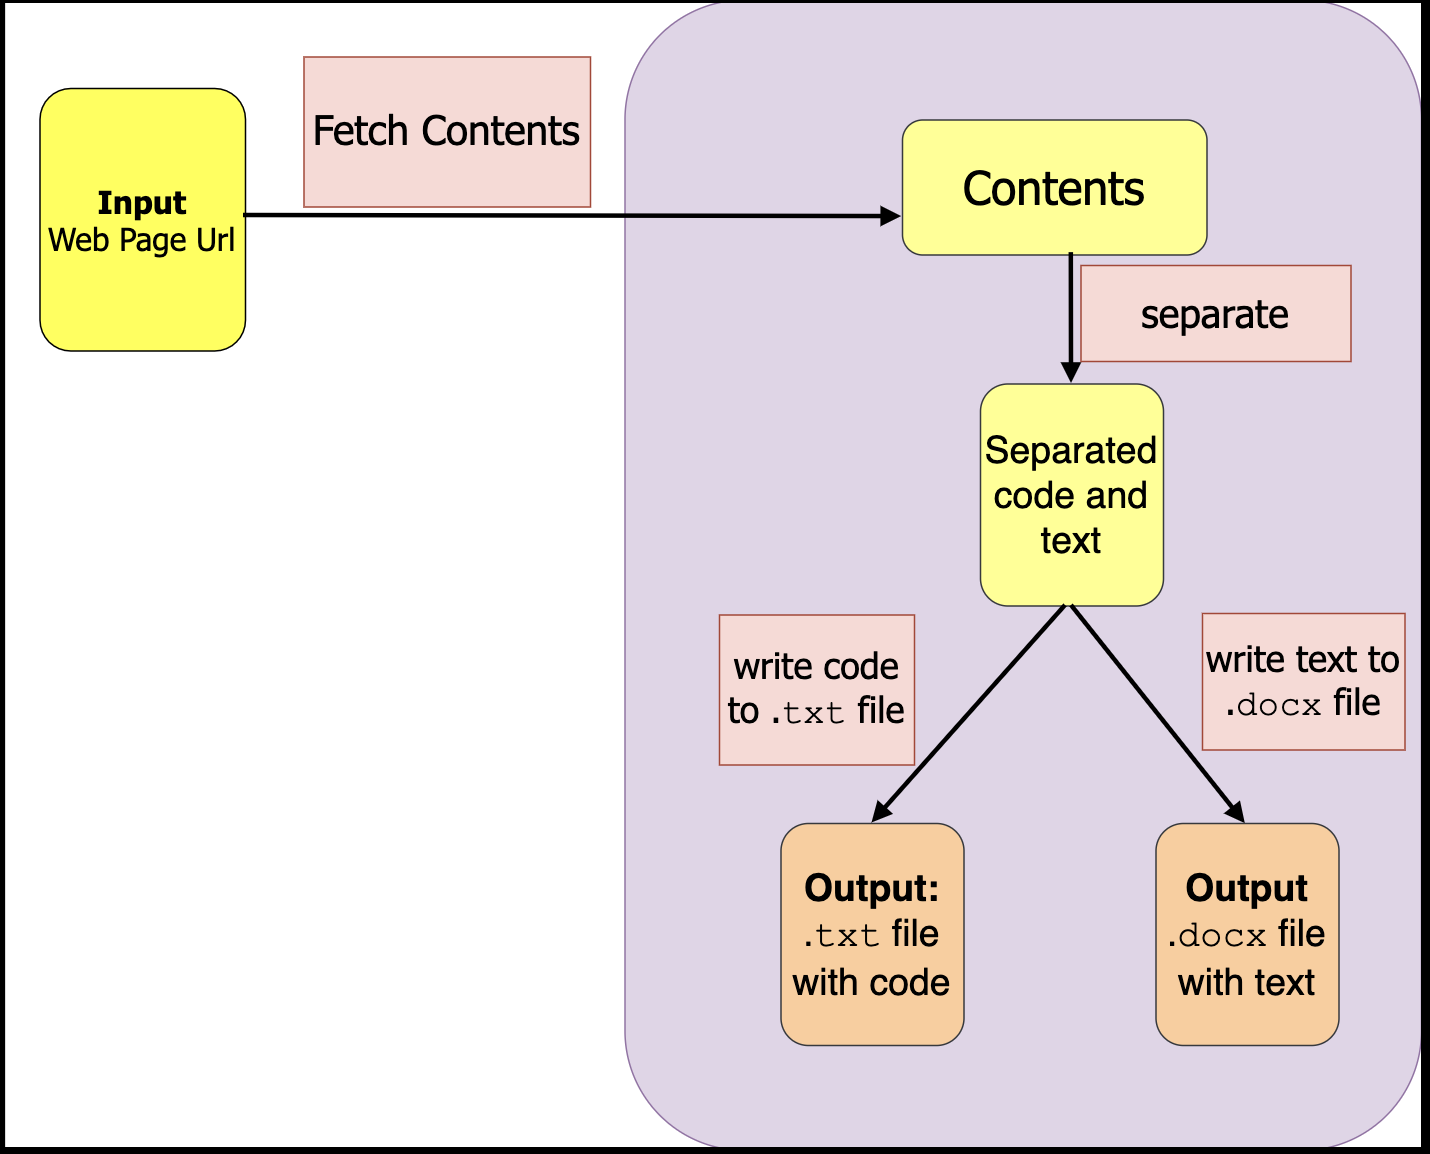
\includegraphics[width=1.0\textwidth]{figures/new-high-arch.png}
    \caption{High-Level Architecture}
    \label{fig:high-level-arch}
\end{figure}


% change this cause it is not consistent with the design later need to make it so that the actual things like the tags and the text tags are in the boxes and the processes are on the arrows. 
The \textbf{high-level architecture} consists of the following:
\begin{enumerate}
    \item Get the contents of the web page specified by the URL.
    % \item Parsing the response obtained from the HTTP libraries into Tags from the \texttt{tagsoup} library.
    % \item Separating the text from the code snippets using the descriptions of each Tag from the above Tags
    \item Separate the code snippets from the text.
    \item Writing the code snippets into a \texttt{.txt} file.
    \item Write the non-code textual content into a \texttt{.docx} file.
\end{enumerate}



\section{High-Level Design}


\begin{figure}[h]
    \centering
    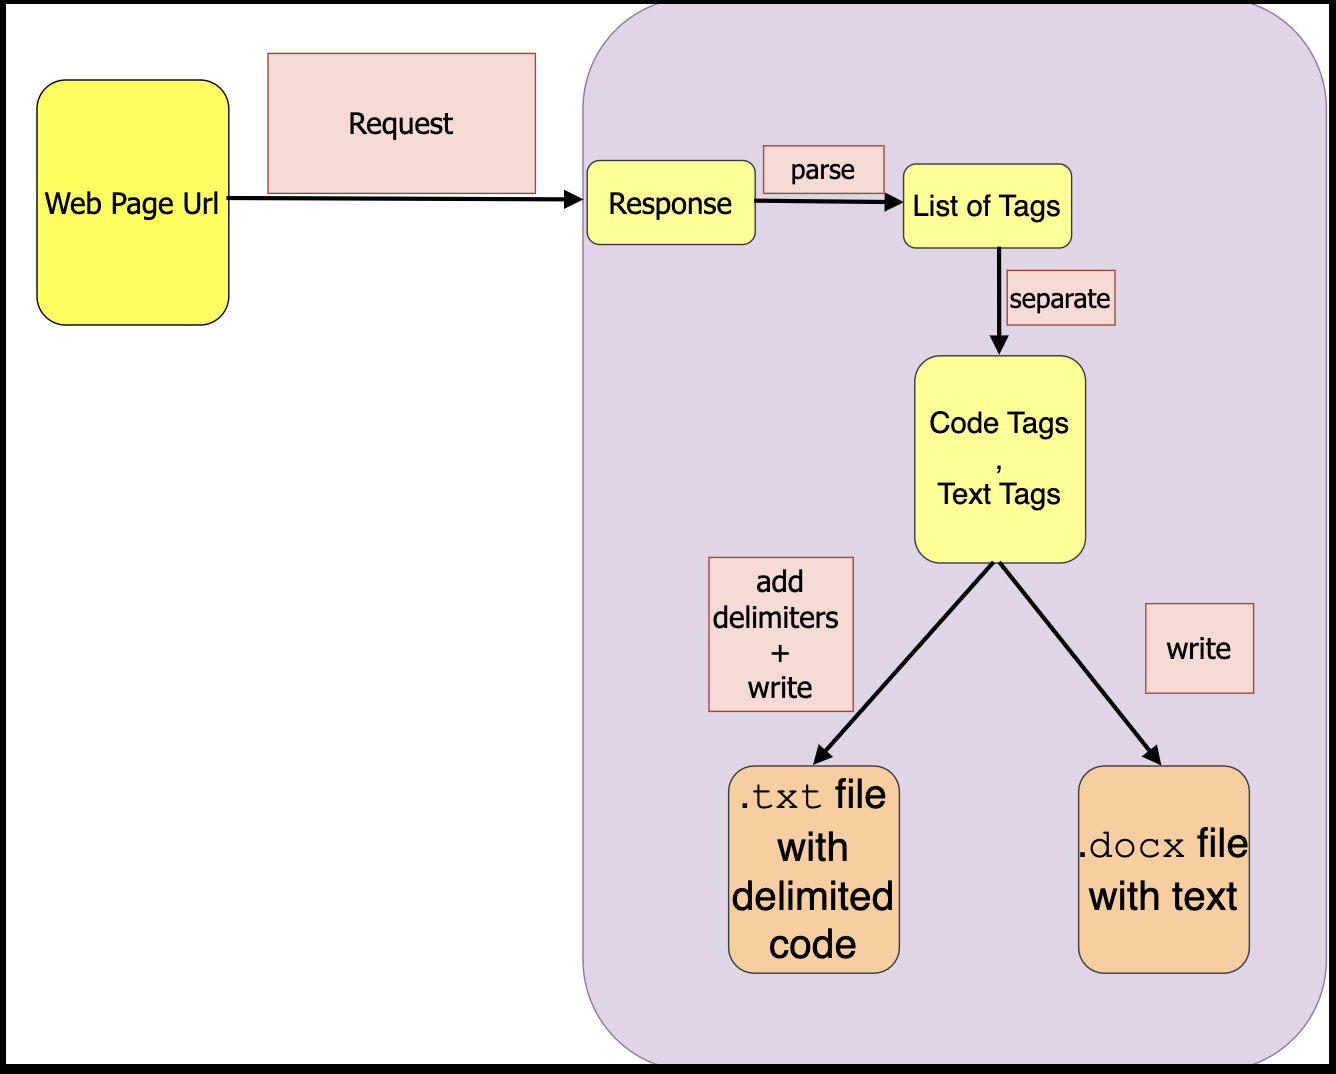
\includegraphics[width=1.0\textwidth]{figures/new-high-design.png}
    \caption{High-Level Design}
    \label{fig:high-level-design}
\end{figure}

A more detailed description of the \textbf{high-level design} which implements the architecture consists of the following:
\begin{enumerate}
    \item Execute an HTTPS request for fetching the HTML contents of the web page
    % \item Parsing the url into a request
    % \item Executing the request with the TLS manager
    \item Get the body i.e. the HTML content from the response received after executing the request
    \item Parse the HTML into a list of Tags according to the \texttt{tagsoup} library
    \item Separate the Tags corresponding to the code from the Tags corresponding to the textual content. By inspecting the HTML, we can see that the code snippets are within \texttt{<pre>} tags, so we need to separate everything enclosed within these tags from the rest of the HTML content. We also remove images. 
    \item Insert delimiters between each different code snippet for formatting purposes. 
    % \item Convert the list of Tag Strings corresponding to the code and to the text each back into an HTML-formatted string, which we then convert into a \texttt{pandoc} document as intermediate representation
    % \item Convert the pandocs into another intermediate string-like format which can then be written into the respective \texttt{.docx} and \texttt{.txt} files
    \item Convert the Tags back to HTML
    \item Write the code snippets to the \ttt{.txt} file
    \item Write the non-code textual content to the \ttt{.docx} file
\end{enumerate}

The lower level implementation details are mentioned in the prototype implementation section.












\chapter {Tools and Languages}
% tech stack
% need to be clear on cabal stack and haskell and stuff


\section{Languages}

Only Haskell was used for the project as mentioned in the problem statement

\section{Tools}

\begin{enumerate}
    \item The Glasgow Haskell Compiler (GHC) is used for compilation.
    \item \href{https://docs.haskellstack.org/en/stable/}{Stack} is used as the build tool. This manages installing project dependencies, building and running the project and testing the project.
    \item \textbf{Libraries}:
    \begin{enumerate}
        \item \texttt{Network.HTTP.Client.TLS} was chosen for handling HTTPS connections in order to use the \texttt{newTlsManager} function
        \item \texttt{Network.HTTP.Client} was chosen for parsing the url into a request, executing the request with the manager, and getting the body from the response. The functions used were \texttt{parseRequest, httpLbs, responseBody} respectively.
        \item \texttt{Tagsoup} was used to parse the HTML into a list of Tag Strings, and then also to convert the separated Tag Strings back into an HTML-formatted string . It was also used in a helper function that inserted a delimiter between the code snippets. The functions used were \texttt{parseTags, isTagOpenName, isTagCloseName, renderTags}, along with the \texttt{TagText} constructor and \texttt{Tag} for \texttt{Tag String}.
        \item \texttt{Pandoc} was used to read the HTML-formatted strings for both the code and the text into intermediate Pandoc representation. Then it was used to write the content into another intermediate string-like representation, which in turn was written into the final files with a standard library. The functions used were \texttt{readHtml, writePlain, writeDocx, runIO}.
        \item \texttt{Data.ByteString.Lazy.Char8} was used to convert the ByteString obtained from the response body into a string for further processing. The function used was \texttt{unpack}
        \item \texttt{Data.ByteString.Lazy} was used to write the ByteString obtained from the \texttt{writeDocx} function from \texttt{pandoc}, into the final \texttt{.docx} file. The function used was \texttt{writeFile}
        \item \texttt{Data.Text.Conversions} was used to convert the separated HTML strings into the \texttt{Text} type defined under \texttt{Data.Text}, so that it could be converted into intermediate pandoc representation by \texttt{readHtml}. The function used was \texttt{convertText}.
        \item \texttt{Data.Text} was used in order to use the \texttt{Text} type
        \item \texttt{Data.Text.IO} was used to write the Text obtained from the \texttt{writePlain} function from \texttt{pandoc}, into the final \texttt{.txt} file. The function used was \texttt{writeFile}
        \item The standard \texttt{Prelude} was used for various operations.
    \end{enumerate} 
\end{enumerate}






\chapter{Test Plan}
% test individual functions 
% for the midterm eval at the end if have time (need to) then can write one big test 

% \section{Tools to be used for Testing}



\section{Test Suite Outline}

\begin{enumerate}
    \item \textbf{Unit Testing : } The following functions can be tested 
    \begin{enumerate}
        \item \texttt{getHTML : }
        \begin{enumerate}
            \item Test if the function returns the correct HTML for various URLs by using sample inputs and outputs.
            \item Test if the function gracefully handles invalid URLs with error handling.
            \item Test if the function handles network errors and HTTPS errors with error handling.
        \end{enumerate}

        \item \texttt{parseTheTags : }
        \begin{enumerate}
            \item Test if the function returns the correct list of Tag Strings for various HTML content.
            \item Test if the function handles malformed HTML and erroneous inputs with error handling.
        \end{enumerate}

        \item \texttt{fillTrue : }
        \begin{enumerate}
            \item Test if the function correctly fills in True values for all elements within any two matching pair of True values corresponding to \texttt{<pre>} tags.
            \item Test if the function handles edge cases with empty lists or single element lists.
        \end{enumerate}

        \item \texttt{insertNewLines : }
        \begin{enumerate}
            \item Test if the function correctly adds the delimiter before every closing \texttt{<pre>} tag.
            \item Test if the function handles cases where there are no \texttt{<pre>} tags, or the Tag String is malformed 
        \end{enumerate}

        \item \texttt{separateTextCode : }
        \begin{enumerate}
            \item Test if the function correctly returns a tuple of two lists where one list has the Tag Strings corresponding to all the content enclosed within \texttt{<pre>} tags, and that the other list has all the other elements, excluding images.
            \item Test edge cases of no \texttt{<pre>} tags, nested \texttt{<pre>} tags
        \end{enumerate}

        \item \texttt{writeToTxt : }
        While File I/O cannot be unit-tested in the traditional sense, we can still manually test the file outputs.
        \begin{enumerate}
            \item Test if the function correctly writes the content of the input Tag String with delimters to the \texttt{.txt} file using sample input output
        \end{enumerate}

        \item \texttt{writeToDocx : }
        While File I/O cannot be unit-tested in the traditional sense, we can still manually test the file outputs.
        \begin{enumerate}
            \item Test if the function correctly writes the content of the input Tag String to the \texttt{.docx} file using sample input output
        \end{enumerate}

    \end{enumerate}
    \item \textbf{Performance Testing : } 
    \begin{enumerate}
        \item Test the time taken for the full system to execute from start to finish
        \item Test the resource consumption of the system
    \end{enumerate}
    \item \textbf{Functional Testing : } \\ Test whether the program meets the requirements by using sample input URLs and sample output files
\end{enumerate}






\chapter{Prototype Implementation Details}
% this can give a broad overview of what the prototype can and cannot do. What the input and output of the prototype look like etc.

\section{Prototype File Structure}

\begin{verbatim}
scraper
|-- app
|   | -- Main.hs (main driver code)
|-- src
|   |-- Lib.hs (implementation of functions)
|-- output_files
|   | -- final_code.txt (delimited code snippets)
|   | -- final_text.docx (textual content)


\end{verbatim}



\section{Prototype features and limitations}

The prototype correctly identifies the code and text portions of the web page and writes them into the \texttt{.txt} and \texttt{.docx} files as per the requirements and specifications. 

\subsubsection{Limitations}



\begin{enumerate}
            \item The prototype has not been robustly tested, verified for correctness or structured to handle errors. However, this can be developed while making the final system since the prototype is already relatively modular.
            \item Since the HTML structure of different web pages can vary, it is not necessary that this particular scraper will work for all web pages. It is designed specifically for the given page and may work for some other pages. But no generalisation can be made about the correctness of its text and code extraction for other pages.
            \item Moreover, it will not necessarily work for web pages with malformed HTML or different structure.
            \item It is not designed to be robust to design changes, which is in line with the \href{https://hackage.haskell.org/package/tagsoup-0.6/src/tagsoup.htm#:~:text=Rule%202%3A%0ADo%20not%20be%20robust%20to%20design%20changes%2C%20do%20not%20even%20consider%20the%20possibility%20when%20writing%20the%20code.}{rule} stated on the \texttt{tagsoup} library's documentation example, since the website's HTML can change in unpredictable ways. If the site's HTML structure changes, for instance if the code snippets change from being enclosed in \texttt{<pre>} tags to \texttt{<code>} tags, then the scraper will not be able to separate out the code from the text and extract them accurately.
            \item It clearly does not work with text sources that are not HTML formatted web pages.
\end{enumerate}



\section{Implementation Details}


\subsection{Main.hs}

In-line with the design, architecture and choice of tools as mentioned above, the prototype obtains the HTML content of the url in line 2 and parses it into Tag Strings in line 3. Then we separate it into code tags and non-code textual tags in lines 4-6. Then we write the Tags to respective files in like 7-8.\\
\\ The core structure of the \texttt{Main.hs} file is
\begin{minted}{haskell}

    1. let url = "https://eli.thegreenplace.net/2018/type-erasure-and-reification/"
    2. response_html <- getHTML url
    3. let parsed_tags = parseTheTags response_html
    4. let separated_text_code = separateTextCode parsed_tags
    5. let preTags             = fst separated_text_code
    6. let nonPreTags          = snd separated_text_code
    7. writeToTxt preTags
    8. writeToDocx nonPreTags

\end{minted}

\subsection{Lib.hs}

\subsubsection{Imports and pragmas}

\begin{minted}[%
 breaklines,
 mathescape,
 linenos,
 numbersep=5pt,
 frame=single,
 numbersep=5pt,
 xleftmargin=0pt,
 ]{haskell}
{-# LANGUAGE OverloadedStrings #-}
import qualified Network.HTTP.Client as Client
import qualified Network.HTTP.Client.TLS as ClientTLS

import qualified Text.HTML.TagSoup as Soup
import Text.Pandoc

import qualified Data.Text.Conversions as TextConv
import qualified Data.Text as T
import qualified Data.Text.IO as TIO
import qualified Data.ByteString.Lazy as LBS
import qualified Data.ByteString.Lazy.Char8 as LBSC

\end{minted}

\subsubsection{getHTML}
\texttt{getHTML} takes the url as input and sets up a new TLS manager with \texttt{newTlsManager}, parses the url with \texttt{parseRequest} and then executes the request with \texttt{httpLbs}. \\ Then it gets the HTML content from the response using \texttt{responseBody}.

\begin{minted}[%
 breaklines,
 mathescape,
 linenos,
 numbersep=5pt,
 frame=single,
 numbersep=5pt,
 xleftmargin=0pt,
 ]{haskell}
getHTML :: String -> IO LBSC.ByteString
getHTML url = do
    mymanager <- ClientTLS.newTlsManager
    myrequest <- Client.parseRequest url
    response <- Client.httpLbs myrequest mymanager
    let response_html = Client.responseBody response
    return response_html
    
\end{minted}







\subsubsection{parseTheTags}
\texttt{parseTheTags} takes the HTML ByteString and parses it into a list of Tag Strings using \texttt{parseTags} from Tagsoup.

\begin{minted}[%
 breaklines,
 mathescape,
 linenos,
 numbersep=5pt,
 frame=single,
 numbersep=5pt,
 xleftmargin=0pt,
 ]{haskell}
parseTheTags :: LBSC.ByteString -> [Soup.Tag String]
parseTheTags response_html = (Soup.parseTags :: String -> [Soup.Tag String]) (LBSC.unpack response_html)
\end{minted}







\subsubsection{fillTrue}
\texttt{fillTrue} is a helper function that fills in True for every element enclosed within a matching pair of True statements corresponding to an opening and closing \texttt{<pre>} tags

\begin{minted}[%
 breaklines,
 mathescape,
 linenos,
 numbersep=5pt,
 frame=single,
 numbersep=5pt,
 xleftmargin=0pt,
 ]{haskell}
fillTrue :: [Bool] -> [Bool]
fillTrue [] = []
fillTrue [a] = [a]
fillTrue (False:False:xs) = False:fillTrue (False:xs)
fillTrue (False:True:xs) = False:fillTrue (True:xs)

-- fill True for elements after a <pre> tag starts
fillTrue (True:False:xs) = True:fillTrue (True:xs) 

-- seeing 2 consecutive Trues denotes end of <pre> tag, so skip them
fillTrue (True:True:xs) = True:True:fillTrue (xs) 
\end{minted}







\subsubsection{insertNewlines}
\texttt{insertNewLines} is a helper function that inserts a TagText for a delimiter before every closing \texttt{<pre>} tag for formatting purposes 

\begin{minted}[%
 breaklines,
 mathescape,
 linenos,
 numbersep=5pt,
 frame=single,
 numbersep=5pt,
 xleftmargin=0pt,
 ]{haskell}
insertNewlines :: [Soup.Tag String] -> [Soup.Tag String]
insertNewlines [] = []
insertNewlines (x:xs) = if (Soup.isTagCloseName "pre" x)
    then Soup.TagText "\n\n=======================\n\n":x:insertNewlines (xs)
    else x:insertNewlines (xs)
\end{minted}


\subsubsection{separateTextCode}
The idea of \texttt{separateTextCode} is as follows. Create a boolean list corresponding to every element of the list of Tag Strings. A boolean list element will be True if a Tag is a \texttt{<pre>} tag or within a \texttt{<pre>} tag. Then zip the boolean list with the original Tag list and get the Tags which have a correponding True value; this is the list of code tags. \\ Now mark elements to be true if the corresponding tags are \texttt{<img>} tags and create an overall boolean list which has false if the tag is not code and not an image. Extract the tags which have a false value; this is the list of non-code textual tags. \\ It essentially solves the parenthesization problem with the \ttt{<pre>} tags.

\begin{minted}[%
 breaklines,
 mathescape,
 linenos,
 numbersep=5pt,
 frame=single,
 numbersep=5pt,
 xleftmargin=0pt,
 ]{haskell}
separateTextCode :: [Soup.Tag String] -> ([Soup.Tag String], [Soup.Tag String])
separateTextCode parsed_tags =
    let bool_mapping_open = Prelude.map (Soup.isTagOpenName "pre") parsed_tags
        bool_mapping_close = Prelude.map (Soup.isTagCloseName "pre") parsed_tags

        -- do element-vise or of the two lists
        bool_mapping1 =  Prelude.zipWith (||) bool_mapping_open bool_mapping_close

        filled_true_pre = fillTrue bool_mapping1
        combined_pre = Prelude.zip filled_true_pre parsed_tags
        preTags = Prelude.map snd (Prelude.filter (fst) combined_pre)

        bool_mapping_img_open = Prelude.map (Soup.isTagOpenName "img") parsed_tags
        bool_mapping_img_close = Prelude.map (Soup.isTagCloseName "img") parsed_tags
        bool_mapping2 =  Prelude.zipWith (||) bool_mapping_img_open bool_mapping_img_close

        bool_mapping =  Prelude.zipWith (||) bool_mapping1 bool_mapping2

        filled_true = fillTrue bool_mapping
        -- zip parsed_tags list with the boolean list and Prelude.filter elements of the first list based on the second list to create tuple list
        combined = Prelude.zip filled_true parsed_tags
        -- get tags of tuples from combined where the boolean is false
        nonPreTags = Prelude.map snd (Prelude.filter (\(a,_) -> not a) combined)

    in (preTags, nonPreTags)


\end{minted}


\subsubsection{Writers to files}
\texttt{writeToTxt} takes the code Tags and renders them as an HTML formatted string after delimiting the snippets. Then the string is converted into the Text type, which is then fed into \texttt{readHtml} which converts it into an intermediate Pandoc format.\\ \texttt{writePlain} converts this pandoc into Text, which is finally written to the \texttt{.txt} file. \\
\\ \texttt{writeToDocx} takes the text Tags and renders them as an HTML formatted string. Then the string is converted into the Text type, which is then fed into \texttt{readHtml} which converts it into an intermediate Pandoc format.\\ \texttt{writeDocx} converts this pandoc into a ByteString, which is finally written to the \texttt{.txt} file. 

\begin{minted}[%
 breaklines,
 mathescape,
 linenos,
 numbersep=5pt,
 frame=single,
 numbersep=5pt,
 xleftmargin=0pt,
 ]{haskell}
writeToTxt :: [Soup.Tag String] -> IO ()
writeToTxt preTags = do
    let htmlPre = Soup.renderTags (insertNewlines preTags)
    pandocPre <- runIO $ readHtml def ( TextConv.convertText (htmlPre :: String ) :: T.Text )

    case pandocPre of
        Right x -> do
            y <- runIO $ writePlain def x
            case y of
                Right direct_pan_pre -> do
                    TIO.writeFile "output_files/final_code.txt" direct_pan_pre

                Left err -> Prelude.putStrLn $ "Error with pandoc writePlain: " ++ show err

        Left err -> Prelude.putStrLn $ "Error parsing pandoc for pre tags: " ++ show err
    
    putStrLn "Completed writing to txt"


writeToDocx :: [Soup.Tag String] -> IO ()
writeToDocx nonPreTags = do
    let htmlNonPre = Soup.renderTags nonPreTags
    pandocNoPre <- runIO $ readHtml def ( TextConv.convertText (htmlNonPre :: String ) :: T.Text )

    case pandocNoPre of
        Right x -> do
            y <- runIO $ writeDocx def x
            case y of
                Right direct_pan -> do
                    LBS.writeFile "output_files/final_text.docx" direct_pan

                Left err -> Prelude.putStrLn $ "Error with pandoc writeDocx: " ++ show err

        Left err -> Prelude.putStrLn $ "Error parsing pandoc for non pre tags: " ++ show err

    putStrLn "Completed writing to docx"

\end{minted}












\chapter{Plan for Completion}
% will test. will do error handling. formal verification and validation stuff and maybe make more robust for other urls also idk. Getting better performance


\begin{itemize}
    \item Implement error handling gracefully wherever possible so that no unhandled errors can occur.
    \item Implement the test suite
    \item Attempt to make the scraper more generalized so that it can work with other websites and other HTML structures.
    \item Document the code well
    \item Explore methods of separating the code from the non-code textual content that are independent of HTML structure. Such methods were mentioned in the analysis and implementation of these methods will make the scraper more generalizable. 
\end{itemize}


















\end{document}